\documentclass[10pt,twocolumn,a4paper]{extarticle}
\usepackage{iftex}
\ifPDFTeX
  \usepackage[T1]{fontenc}\usepackage[utf8]{inputenc}
  \usepackage[french]{babel}\usepackage{lmodern}
\else
  \usepackage{fontspec}
  \usepackage{polyglossia}\setdefaultlanguage{french}
\fi
\usepackage{microtype,float}
\usepackage[a4paper,margin=1.45cm,columnsep=0.6cm]{geometry}
\usepackage{amsmath,amssymb,bm,booktabs,graphicx,enumitem,titlesec,xcolor,caption}
\setlist[itemize]{nosep,leftmargin=1.1em,label=\textbullet}
\titleformat{\section}{\normalsize\bfseries\sffamily}{\thesection}{0.5em}{}
\titlespacing*{\section}{0pt}{6pt}{2pt}
\captionsetup{font=footnotesize,labelfont=bf,skip=3pt}
\setlength{\parskip}{2pt}\setlength{\parindent}{0pt}
\setlength{\abovedisplayskip}{3pt}\setlength{\belowdisplayskip}{3pt}
\setlength{\abovedisplayshortskip}{2pt}\setlength{\belowdisplayshortskip}{2pt}
\setlength{\textfloatsep}{6pt}\setlength{\dbltextfloatsep}{6pt}\setlength{\floatsep}{5pt}
\newcommand{\code}[1]{\texttt{\small #1}}
\pagestyle{empty}

\begin{document}
\twocolumn[{%
\begin{center}
{\Large\bfseries\sffamily Stratégie systématique multi-asset : des données au backtest}\\[3pt]
{\small Jean Philippe N'Dri \quad\textbullet\quad 6 octobre 2026 \quad\textbullet\quad code : \code{multiasset-strat}, bâti sur \code{portopt}}
\end{center}
\vspace{-2pt}
\noindent\small\textbf{Résumé.} La stratégie sélectionne chaque mois 10 lignes parmi 132 actifs (actions US, ETF, obligations, matières premières) à l'aide de signaux de prix, les pondère par budget de risque et limite les rotations pour tenir compte de frais fixes par ordre. Sur 2018--2026, période non utilisée pour choisir les signaux, le Sharpe net est de 1{,}15 contre 0{,}82 pour un 60/40. Ce résultat est surestimé par un biais de survie non corrigé.
\vspace{6pt}
}]

\section{Données et univers}
Les prix de clôture ajustés (dividendes réinvestis) viennent de Yahoo Finance depuis 2008 et sont convertis en rendements simples quotidiens $r_{i,t}=P_{i,t}/P_{i,t-1}-1$. L'univers compte quatre poches et un actif refuge :
\begin{itemize}
\item \textbf{Actions} (96) : grandes capitalisations du S\&P~500 et du Nasdaq~100 ;
\item \textbf{ETF} (21) : indices, facteurs, thématiques, multi-asset ;
\item \textbf{Obligations} (8) et \textbf{matières premières} (7) ;
\item \textbf{Cash} : \code{SHY}, qui reçoit le capital des emplacements vides.
\end{itemize}
Un actif n'est éligible à la date $t$ que s'il possède 252 rendements consécutifs avant $t$ : les titres cotés tardivement entrent donc naturellement. Les ETF sont des proxys américains ; l'exécution réelle passe par des équivalents UCITS.

\section{Signaux}
Tous les signaux sont calculés sur la fenêtre $[t-252,\,t)$, sans information postérieure à $t$. Treize signaux de prix tirés de la littérature ont été testés un par un, par poche, sur 2009--2017, puis vérifiés une seule fois sur 2018--2026. Cinq sont retenus.

\textbf{Tendance} (actions, ETF, matières premières) :
\begin{align*}
\text{mom}_{12\text{-}1} &= \frac{P_{t-21}}{P_{t-252}}-1, &
\text{mom}_{6\text{-}1} &= \frac{P_{t-21}}{P_{t-126}}-1,\\
\text{ma}_{200} &= \frac{P_t}{\mathrm{SMA}_{200}}-1, &
\text{ma}_{50/200} &= \frac{\mathrm{SMA}_{50}}{\mathrm{SMA}_{200}}-1.
\end{align*}
\textbf{Retour à la moyenne} (obligations) :
\[
\text{boll}_{20} = -\,\frac{P_t-\mathrm{SMA}_{20}}{\sigma_{20}(P)}.
\]
Chaque signal $x_{i,k}$ est winsorisé à 1\,\%/99\,\% puis standardisé \emph{à l'intérieur de sa poche} $g$, et le score est la moyenne des $K_g$ signaux de la poche :
\[
z_{i,k}=\frac{x_{i,k}-\mu^{(g)}_k}{\sigma^{(g)}_k},\qquad S_i=\frac{1}{K_g}\sum_{k=1}^{K_g} z_{i,k}.
\]
La standardisation par poche évite de comparer le momentum d'une action à celui d'une obligation, dont les dispersions n'ont rien de commun. S'ajoute un \textbf{filtre absolu} : un actif n'est achetable que si $P_t>\mathrm{SMA}_{200}$.

La faible volatilité, présente dans la première version du score, a été retirée : son coefficient d'information est négatif sur les actions et les ETF, sur les deux sous-périodes.

\section{Sélection}
Le portefeuille détient 5 actions, 2 ETF, 2 obligations et 1 matière première. Dans chaque poche, on retient les meilleurs scores parmi les actifs passant le filtre. Trois règles limitent les rotations :
\begin{itemize}
\item \textbf{hystérésis} : une ligne détenue ne sort que si elle casse sa tendance ou quitte les 40\,\% supérieurs de sa poche ;
\item \textbf{deux sorties au plus} par rebalancement, les tendances cassées d'abord ;
\item un emplacement sans candidat est placé sur \code{SHY}.
\end{itemize}

\section{Allocation}
Les poids des $n$ lignes retenues résolvent un problème de budget de risque. Avec $\bm\Sigma$ la covariance de Ledoit--Wolf estimée sur la fenêtre, la contribution relative de la ligne $i$ est
\[
\mathrm{RC}_i=\frac{w_i\,(\bm\Sigma\bm w)_i}{\bm w^{\top}\bm\Sigma\bm w},\qquad \sum_i \mathrm{RC}_i=1,
\]
et l'on impose $\mathrm{RC}_i=b_i$, où les budgets par poche valent 40\,\% pour les actions, 24\,\% pour les ETF, 24\,\% pour les obligations et 12\,\% pour les matières premières, répartis également entre les lignes d'une poche. La solution est obtenue par descente de coordonnées sur la formulation convexe de Spinu,
\[
\bm y^{\star}=\arg\min_{\bm y>0}\ \tfrac12\,\bm y^{\top}\bm\Sigma\bm y-\sum_i b_i\ln y_i,\qquad \bm w=\frac{\bm y^{\star}}{\bm 1^{\top}\bm y^{\star}}.
\]
Les poids sont ensuite bornés ($5\,\%\le w_i\le 20\,\%$, plancher de 3\,\% pour une action). Comme ces bornes déforment les budgets, le budget des actions est ré-imposé comme plafond par bissection sur un facteur de réduction de la poche.

\section{Contraintes de turnover}
Soit $\bm w^{-}$ le portefeuille détenu (poids dérivés) et $\bm w^{\star}$ la cible. Les frais étant fixes par ordre, le coût dépend du \emph{nombre} d'ordres et non du montant traité. L'exécution applique donc :
\begin{itemize}
\item une \textbf{bande de non-transaction} : pas d'ordre si $|w^{\star}_i-w^{-}_i|<2$ points ;
\item un \textbf{plafond} $\tau_t=\sum_i|w_{i,t}-w^{-}_{i,t}|\le 40\,\%$, en renonçant d'abord aux plus petits ajustements.
\end{itemize}
Les bornes de poids priment sur le plafond, qui reste souple pour la dernière rotation.

\begin{figure*}[t]
\centering
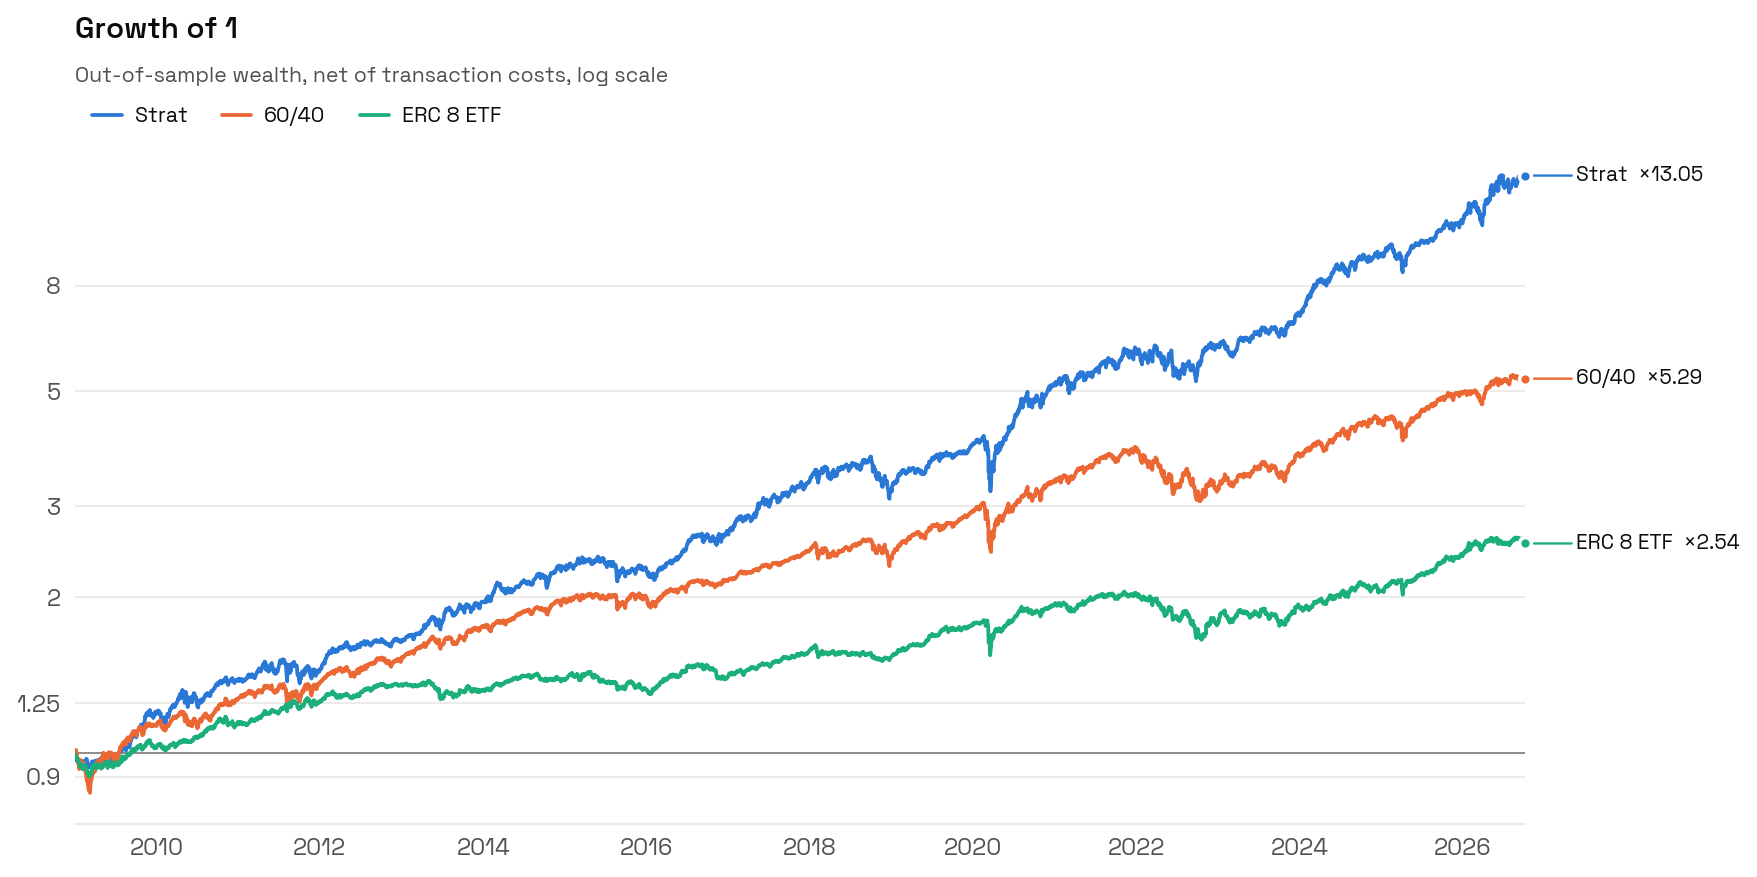
\includegraphics[width=0.8\textwidth]{wealth.png}
\caption{Valeur de 1 investi, nette de frais, échelle logarithmique.}
\end{figure*}

\section{Backtest}
Le backtest est \emph{walk-forward} : à chaque date $t$ de la grille (tous les 21 jours de bourse), les poids sont calculés sur $r_{[t-252,\,t)}$ et appliqués à partir de $r_t$, puis dérivent librement jusqu'au rebalancement suivant. Le coût payé en $t$ est
\[
c_t=s\,\tau_t+\frac{f\,n^{\text{ordres}}_t}{\mathrm{NAV}_t},
\]
avec $s=5$~pb, $f=1$~\texteuro{} par ordre et $\mathrm{NAV}_0=10\,317$~\texteuro{}. Un frais fixe pèse donc d'autant plus que le compte est petit. Deux références subissent les mêmes frais : un 60/40 (\code{SPY}/\code{IEF}) et une parité de risque sur 8 ETF sans signal.

\section{Résultats}
\begin{table}[H]
\centering\footnotesize
\begin{tabular}{@{}lrrr@{}}
\toprule
Net de frais & Stratégie & 60/40 & ERC 8 ETF\\
\midrule
\multicolumn{4}{@{}l}{\emph{2009--2026}}\\
Rendement annualisé & 15{,}6\,\% & 9{,}9\,\% & 5{,}4\,\%\\
Volatilité & 12{,}4\,\% & 10{,}3\,\% & 7{,}2\,\%\\
Sharpe & 1{,}23 & 0{,}96 & 0{,}76\\
Perte maximale & $-21{,}9\,\%$ & $-21{,}5\,\%$ & $-19{,}4\,\%$\\
\midrule
\multicolumn{4}{@{}l}{\emph{2018--2026, hors échantillon}}\\
Rendement annualisé & 16{,}9\,\% & 9{,}2\,\% & 5{,}6\,\%\\
Volatilité & 14{,}5\,\% & 11{,}5\,\% & 8{,}1\,\%\\
Sharpe & 1{,}15 & 0{,}82 & 0{,}71\\
\bottomrule
\end{tabular}
\caption{Performance nette de frais. Les signaux ont été choisis sur 2009--2017.}
\end{table}
Sur 2018--2026, l'écart avec le 60/40 est de 7{,}2 points par an ($t=2{,}4$). La stratégie passe en moyenne 4{,}3 ordres par rebalancement, pour 0{,}4\,\% de frais annuels et un turnover de 387\,\% par an.

\textbf{Contrôles de risque.} Le portefeuille ne dépasse jamais 10 lignes ni 21{,}7\,\% par ligne. La poche actions porte en moyenne 44\,\% du risque (cible 40\,\%, maximum 59\,\% entre deux rebalancements). La variance ex ante se décompose en 62\,\% de bêta de marché et 26\,\% de risque spécifique, dont 12\,\% pour les actions. La pire perte journalière due à une seule ligne est de 2{,}3 points de NAV. Le plafond de turnover est dépassé dans 16{,}5\,\% des rebalancements.


\section{Limites}
\begin{itemize}
\item \textbf{Biais de survie.} Les actions sont les grandes capitalisations d'aujourd'hui. Un signal de tendance appliqué à des survivantes est flatté, d'un montant non chiffré.
\item \textbf{Preuve statistique faible.} Aucun signal isolé ne résiste à la correction de Benjamini--Hochberg sur les 52 tests (meilleure $q$-valeur : 0{,}46). L'effet sur les actions vit dans la queue : le top~5 surperforme alors que l'IC de rang est nul.
\item \textbf{Concentration sectorielle.} Aucune contrainte par secteur : au 5 octobre 2026, les cinq actions retenues sont des semi-conducteurs.
\item \textbf{Devise.} Backtest en dollars, sans effet de change EUR/USD.
\end{itemize}
\end{document}
